\documentclass[book,11pt]{IEEEtran} 
 \usepackage{setspace} 
 \usepackage{gensymb} 
 \singlespacing 
 \usepackage[cmex10]{amsmath} 
 \usepackage{amsthm} 
 \usepackage{mathrsfs} 
 \usepackage{txfonts} 
 \usepackage{stfloats} 
 \usepackage{bm} 
 \usepackage{cite} 
 \usepackage{cases} 
 \usepackage{subfig} 
 \usepackage{longtable} 
 \usepackage{multirow} 
 \usepackage{enumitem} 
 \usepackage{mathtools} 
 \usepackage{tikz} 
 \usepackage{circuitikz} 
 \usepackage{verbatim} 
 \usepackage[breaklinks=true]{hyperref} 
 \usepackage{tkz-euclide} % loads  TikZ and tkz-base 
 \usepackage{listings} 
 \usepackage{color}     
 \usepackage{array}     
 \usepackage{longtable} 
 \usepackage{calc}      
 \usepackage{multirow}  
 \usepackage{hhline}    
 \usepackage{ifthen}    
 \usepackage{lscape}      
 \usepackage{chngcntr} 
 \usepackage{float} 
 \DeclareMathOperator*{\Res}{Res} 
 \renewcommand\thesection{\arabic{section}} 
 \renewcommand\thesubsection{\thesection.\arabic{subsection}} 
 \renewcommand\thesubsubsection{\thesubsection.\arabic{subsubsection}} 
  
 \renewcommand\thesectiondis{\arabic{section}} 
 \renewcommand\thesubsectiondis{\thesectiondis.\arabic{subsection}} 
 \renewcommand\thesubsubsectiondis{\thesubsectiondis.\arabic{subsubsection}} 
 \renewcommand\thetable{\arabic{table}} 
 % correct bad hyphenation here 
 \hyphenation{op-tical net-works semi-conduc-tor} 
 \def\inputGnumericTable{}                                 %% 
  
 \lstset{ 
 %language=C, 
 frame=single,  
 breaklines=true, 
 columns=fullflexible 
 } 
 %\lstset{ 
 %language=tex, 
 %frame=single,  
 %breaklines=true 
 %} 
  
 \begin{document} 
 \newtheorem{theorem}{Theorem}[section] 
 \newtheorem{problem}{Problem} 
 \newtheorem{proposition}{Proposition}[section] 
 \newtheorem{lemma}{Lemma}[section] 
 \newtheorem{corollary}[theorem]{Corollary} 
 \newtheorem{example}{Example}[section] 
 \newtheorem{definition}[problem]{Definition} 
 \newcommand{\BEQA}{\begin{eqnarray}} 
 \newcommand{\EEQA}{\end{eqnarray}} 
 \newcommand{\define}{\stackrel{\triangle}{=}} 
 \bibliographystyle{IEEEtran} 
 \providecommand{\mbf}{\mathbf} 
 \providecommand{\pr}[1]{\ensuremath{\Pr\left(#1\right)}} 
 \providecommand{\qfunc}[1]{\ensuremath{Q\left(#1\right)}} 
 \providecommand{\sbrak}[1]{\ensuremath{{}\left[#1\right]}} 
 \providecommand{\lsbrak}[1]{\ensuremath{{}\left[#1\right.}} 
 \providecommand{\rsbrak}[1]{\ensuremath{{}\left.#1\right]}} 
 \providecommand{\brak}[1]{\ensuremath{\left(#1\right)}} 
 \providecommand{\lbrak}[1]{\ensuremath{\left(#1\right.}} 
 \providecommand{\rbrak}[1]{\ensuremath{\left.#1\right)}} 
 \providecommand{\cbrak}[1]{\ensuremath{\left\{#1\right\}}} 
 \providecommand{\lcbrak}[1]{\ensuremath{\left\{#1\right.}} 
 \providecommand{\rcbrak}[1]{\ensuremath{\left.#1\right\}}} 
 \theoremstyle{remark} 
 \newtheorem{rem}{Remark} 
 \newcommand{\sgn}{\mathop{\mathrm{sgn}}} 
 \providecommand{\abs}[1]{\left\vert#1\right\vert} 
 \providecommand{\res}[1]{\Res\displaylimits_{#1}}  
 \providecommand{\norm}[1]{\left\lVert#1\right\rVert} 
 \providecommand{\mtx}[1]{\mathbf{#1}} 
 \providecommand{\mean}[1]{E\left[ #1 \right]} 
 \providecommand{\fourier}{\overset{\mathcal{F}}{ \rightleftharpoons}} 
 \providecommand{\system}[1]{\overset{\mathcal{#1}}{ \longleftrightarrow}} 
 \newcommand{\solution}{\noindent \textbf{Solution: }} 
 \newcommand{\cosec}{\,\text{cosec}\,} 
 \providecommand{\dec}[2]{\ensuremath{\overset{#1}{\underset{#2}{\gtrless}}}} 
 \newcommand{\myvec}[1]{\ensuremath{\begin{pmatrix}#1\end{pmatrix}}} 
 \newcommand{\mydet}[1]{\ensuremath{\begin{vmatrix}#1\end{vmatrix}}} 
 \let\vec\mathbf 
 \def\putbox#1#2#3{\makebox[0in][l]{\makebox[#1][l]{}\raisebox{\baselineskip}[0in][0in]{\raisebox{#2}[0in][0in]{#3}}}} 
      \def\rightbox#1{\makebox[0in][r]{#1}} 
      \def\centbox#1{\makebox[0in]{#1}} 
      \def\topbox#1{\raisebox{-\baselineskip}[0in][0in]{#1}} 
      \def\midbox#1{\raisebox{-0.5\baselineskip}[0in][0in]{#1}} 
  
 \vspace{3cm}
Questions-1.1.1,1.1.4,1.1.5
\begin{align}
\vec{A}&=\myvec{1\\-1},
\vec{B}=\myvec{-2\\2},
\vec{C}=\myvec{-5\\-3}
\end{align}
\begin{table}[!ht]
        \centering
        %%%%%%%%%%%%%%%%%%%%%%%%%%%%%%%%%%%%%%%%%%%%%%%%%%%%%%%%%%%%%%%%%%%%%%
%%                                                                  %%
%%  This is the header of a LaTeX2e file exported from Gnumeric.    %%
%%                                                                  %%
%%  This file can be compiled as it stands or included in another   %%
%%  LaTeX document. The table is based on the longtable package so  %%
%%  the longtable options (headers, footers...) can be set in the   %%
%%  preamble section below (see PRAMBLE).                           %%
%%                                                                  %%
%%  To include the file in another, the following two lines must be %%
%%  in the including file:                                          %%
%%        \def\inputGnumericTable{}                                 %%
%%  at the beginning of the file and:                               %%
%%        \input{name-of-this-file.tex}                             %%
%%  where the table is to be placed. Note also that the including   %%
%%  file must use the following packages for the table to be        %%
%%  rendered correctly:                                             %%
%%    \usepackage[latin1]{inputenc}                                 %%
%%    \usepackage{color}                                            %%
%%    \usepackage{array}                                            %%
%%    \usepackage{longtable}                                        %%
%%    \usepackage{calc}                                             %%
%%    \usepackage{multirow}                                         %%
%%    \usepackage{hhline}                                           %%
%%    \usepackage{ifthen}                                           %%
%%  optionally (for landscape tables embedded in another document): %%
%%    \usepackage{lscape}                                           %%
%%                                                                  %%
%%%%%%%%%%%%%%%%%%%%%%%%%%%%%%%%%%%%%%%%%%%%%%%%%%%%%%%%%%%%%%%%%%%%%%



%%  This section checks if we are begin input into another file or  %%
%%  the file will be compiled alone. First use a macro taken from   %%
%%  the TeXbook ex 7.7 (suggestion of Han-Wen Nienhuys).            %%
\def\ifundefined#1{\expandafter\ifx\csname#1\endcsname\relax}


%%  Check for the \def token for inputed files. If it is not        %%
%%  defined, the file will be processed as a standalone and the     %%
%%  preamble will be used.                                          %%
\ifundefined{inputGnumericTable}

%%  We must be able to close or not the document at the end.        %%
	\def\gnumericTableEnd{\end{document}}


%%%%%%%%%%%%%%%%%%%%%%%%%%%%%%%%%%%%%%%%%%%%%%%%%%%%%%%%%%%%%%%%%%%%%%
%%                                                                  %%
%%  This is the PREAMBLE. Change these values to get the right      %%
%%  paper size and other niceties.                                  %%
%%                                                                  %%
%%%%%%%%%%%%%%%%%%%%%%%%%%%%%%%%%%%%%%%%%%%%%%%%%%%%%%%%%%%%%%%%%%%%%%

	\documentclass[12pt%
			  %,landscape%
                    ]{report}
       \usepackage[latin1]{inputenc}
       \usepackage{fullpage}
       \usepackage{color}
       \usepackage{array}
       \usepackage{longtable}
       \usepackage{calc}
       \usepackage{multirow}
       \usepackage{hhline}
       \usepackage{ifthen}

	\begin{document}


%%  End of the preamble for the standalone. The next section is for %%
%%  documents which are included into other LaTeX2e files.          %%
\else

%%  We are not a stand alone document. For a regular table, we will %%
%%  have no preamble and only define the closing to mean nothing.   %%
    \def\gnumericTableEnd{}

%%  If we want landscape mode in an embedded document, comment out  %%
%%  the line above and uncomment the two below. The table will      %%
%%  begin on a new page and run in landscape mode.                  %%
%       \def\gnumericTableEnd{\end{landscape}}
%       \begin{landscape}


%%  End of the else clause for this file being \input.              %%
\fi

%%%%%%%%%%%%%%%%%%%%%%%%%%%%%%%%%%%%%%%%%%%%%%%%%%%%%%%%%%%%%%%%%%%%%%
%%                                                                  %%
%%  The rest is the gnumeric table, except for the closing          %%
%%  statement. Changes below will alter the table's appearance.     %%
%%                                                                  %%
%%%%%%%%%%%%%%%%%%%%%%%%%%%%%%%%%%%%%%%%%%%%%%%%%%%%%%%%%%%%%%%%%%%%%%

\providecommand{\gnumericmathit}[1]{#1} 
%%  Uncomment the next line if you would like your numbers to be in %%
%%  italics if they are italizised in the gnumeric table.           %%
%\renewcommand{\gnumericmathit}[1]{\mathit{#1}}
\providecommand{\gnumericPB}[1]%
{\let\gnumericTemp=\\#1\let\\=\gnumericTemp\hspace{0pt}}
 \ifundefined{gnumericTableWidthDefined}
        \newlength{\gnumericTableWidth}
        \newlength{\gnumericTableWidthComplete}
        \newlength{\gnumericMultiRowLength}
        \global\def\gnumericTableWidthDefined{}
 \fi
%% The following setting protects this code from babel shorthands.  %%
 \ifthenelse{\isundefined{\languageshorthands}}{}{\languageshorthands{english}}
%%  The default table format retains the relative column widths of  %%
%%  gnumeric. They can easily be changed to c, r or l. In that case %%
%%  you may want to comment out the next line and uncomment the one %%
%%  thereafter                                                      %%
\providecommand\gnumbox{\makebox[0pt]}
%%\providecommand\gnumbox[1][]{\makebox}

%% to adjust positions in multirow situations                       %%
\setlength{\bigstrutjot}{\jot}
\setlength{\extrarowheight}{\doublerulesep}

%%  The \setlongtables command keeps column widths the same across  %%
%%  pages. Simply comment out next line for varying column widths.  %%
\setlongtables

\setlength\gnumericTableWidth{%
	75pt+%
	75pt+%
	140pt+%
	75pt+%
0pt}
\def\gumericNumCols{4}
\setlength\gnumericTableWidthComplete{\gnumericTableWidth+%
         \tabcolsep*\gumericNumCols*2+\arrayrulewidth*\gumericNumCols}
\ifthenelse{\lengthtest{\gnumericTableWidthComplete > \linewidth}}%
         {\def\gnumericScale{1*\ratio{\linewidth-%
                        \tabcolsep*\gumericNumCols*2-%
                        \arrayrulewidth*\gumericNumCols}%
{\gnumericTableWidth}}}%
{\def\gnumericScale{1}}

%%%%%%%%%%%%%%%%%%%%%%%%%%%%%%%%%%%%%%%%%%%%%%%%%%%%%%%%%%%%%%%%%%%%%%
%%                                                                  %%
%% The following are the widths of the various columns. We are      %%
%% defining them here because then they are easier to change.       %%
%% Depending on the cell formats we may use them more than once.    %%
%%                                                                  %%
%%%%%%%%%%%%%%%%%%%%%%%%%%%%%%%%%%%%%%%%%%%%%%%%%%%%%%%%%%%%%%%%%%%%%%

\ifthenelse{\isundefined{\gnumericColK}}{\newlength{\gnumericColK}}{}\settowidth{\gnumericColK}{\begin{tabular}{@{}p{75pt*\gnumericScale}@{}}x\end{tabular}}
\ifthenelse{\isundefined{\gnumericColL}}{\newlength{\gnumericColL}}{}\settowidth{\gnumericColL}{\begin{tabular}{@{}p{75pt*\gnumericScale}@{}}x\end{tabular}}
\ifthenelse{\isundefined{\gnumericColM}}{\newlength{\gnumericColM}}{}\settowidth{\gnumericColM}{\begin{tabular}{@{}p{140pt*\gnumericScale}@{}}x\end{tabular}}
\ifthenelse{\isundefined{\gnumericColN}}{\newlength{\gnumericColN}}{}\settowidth{\gnumericColN}{\begin{tabular}{@{}p{75pt*\gnumericScale}@{}}x\end{tabular}}

\begin{tabular}[c]{%
	b{\gnumericColK}%
	b{\gnumericColL}%
	b{\gnumericColM}%
	b{\gnumericColN}%
	}

%%%%%%%%%%%%%%%%%%%%%%%%%%%%%%%%%%%%%%%%%%%%%%%%%%%%%%%%%%%%%%%%%%%%%%
%%  The longtable options. (Caption, headers... see Goosens, p.124) %%
%	\caption{The Table Caption.}             \\	%
% \hline	% Across the top of the table.
%%  The rest of these options are table rows which are placed on    %%
%%  the first, last or every page. Use \multicolumn if you want.    %%

%%  Header for the first page.                                      %%
%	\multicolumn{4}{c}{The First Header} \\ \hline 
%	\multicolumn{1}{c}{colTag}	%Column 1
%	&\multicolumn{1}{c}{colTag}	%Column 2
%	&\multicolumn{1}{c}{colTag}	%Column 3
%	&\multicolumn{1}{c}{colTag}	\\ \hline %Last column
%	\endfirsthead

%%  The running header definition.                                  %%
%	\hline
%	\multicolumn{4}{l}{\ldots\small\slshape continued} \\ \hline
%	\multicolumn{1}{c}{colTag}	%Column 1
%	&\multicolumn{1}{c}{colTag}	%Column 2
%	&\multicolumn{1}{c}{colTag}	%Column 3
%	&\multicolumn{1}{c}{colTag}	\\ \hline %Last column
%	\endhead

%%  The running footer definition.                                  %%
%	\hline
%	\multicolumn{4}{r}{\small\slshape continued\ldots} \\
%	\endfoot

%%  The ending footer definition.                                   %%
%	\multicolumn{4}{c}{That's all folks} \\ \hline 
%	\endlastfoot
%%%%%%%%%%%%%%%%%%%%%%%%%%%%%%%%%%%%%%%%%%%%%%%%%%%%%%%%%%%%%%%%%%%%%%

\hhline{|-|-|-~}
	 \multicolumn{1}{|p{\gnumericColK}|}%
	{\gnumericPB{\raggedright}\gnumbox[l]{Parameters}}
	&\multicolumn{1}{p{\gnumericColL}|}%
	{\gnumericPB{\raggedright}\gnumbox[l]{Value}}
	&\multicolumn{1}{p{\gnumericColM}|}%
	{\gnumericPB{\raggedright}\gnumbox[l]{Description}}
	&
\\
\hhline{|---|~}
	 \multicolumn{1}{|p{\gnumericColK}|}%
	{\gnumericPB{\raggedright}\gnumbox[l]{m1}}
	&\multicolumn{1}{p{\gnumericColL}|}%
	{\gnumericPB{\raggedright}\gnumbox[l]{\myvec{-3\\3}}}
	&\multicolumn{1}{p{\gnumericColM}|}%
	{\gnumericPB{\raggedright}\gnumbox[l]{Slope of AB}}
	&
\\
\hhline{|---|~}
	 \multicolumn{1}{|p{\gnumericColK}|}%
	{\gnumericPB{\raggedright}\gnumbox[l]{m2}}
	&\multicolumn{1}{p{\gnumericColL}|}%
	{\gnumericPB{\raggedright}\gnumbox[l]{\myvec{-3\\-5}}}
	&\multicolumn{1}{p{\gnumericColM}|}%
	{\gnumericPB{\raggedright}\gnumbox[l]{Slope of BC}}
	&
\\
\hhline{|---|~}
	 \multicolumn{1}{|p{\gnumericColK}|}%
	{\gnumericPB{\raggedright}\gnumbox[l]{m3}}
	&\multicolumn{1}{p{\gnumericColL}|}%
	{\gnumericPB{\raggedright}\gnumbox[l]{\myvec{6\\2}}}
	&\multicolumn{1}{p{\gnumericColM}|}%
	{\gnumericPB{\raggedright}\gnumbox[l]{Slope of CA}}
	&
\\
\hhline{|---|~}
	 \multicolumn{1}{|p{\gnumericColK}|}%
	{\gnumericPB{\raggedright}\gnumbox[l]{\norm{\vec{B}-\vec{A}}}}
	&\multicolumn{1}{p{\gnumericColL}|}%
	{\gnumericPB{\raggedleft}\gnumbox[r]{4.24}}
	&\multicolumn{1}{p{\gnumericColM}|}%
	{\gnumericPB{\raggedright}\gnumbox[l]{Length of AB}}
	&
\\
\hhline{|---|~}
	 \multicolumn{1}{|p{\gnumericColK}|}%
	{\gnumericPB{\raggedright}\gnumbox[l]{\norm{\vec{C}-\vec{B}}}}
	&\multicolumn{1}{p{\gnumericColL}|}%
	{\gnumericPB{\raggedleft}\gnumbox[r]{5.83}}
	&\multicolumn{1}{p{\gnumericColM}|}%
	{\gnumericPB{\raggedright}\gnumbox[l]{Length of BC}}
	&
\\
\hhline{|---|~}
	 \multicolumn{1}{|p{\gnumericColK}|}%
	{\gnumericPB{\raggedright}\gnumbox[l]{\norm{\vec{A}-\vec{C}}}}
	&\multicolumn{1}{p{\gnumericColL}|}%
	{\gnumericPB{\raggedleft}\gnumbox[r]{6.32}}
	&\multicolumn{1}{p{\gnumericColM}|}%
	{\gnumericPB{\raggedright}\gnumbox[l]{Length of CA}}
	&
\\
\hhline{|---|~}
	 \multicolumn{1}{|p{\gnumericColK}|}%
	{\gnumericPB{\raggedright}\gnumbox[l]{Rank}}
	&\multicolumn{1}{p{\gnumericColL}|}%
	{\gnumericPB{\raggedleft}\gnumbox[r]{3}}
	&\multicolumn{1}{p{\gnumericColM}|}%
	{\gnumericPB{\raggedright}\gnumbox[l]{Non-collinear}}
	&
\\
\hhline{|---|~}
	 \multicolumn{1}{|p{\gnumericColK}|}%
	{\gnumericPB{\raggedright}\gnumbox[l]{n1}}
	&\multicolumn{1}{p{\gnumericColL}|}%
	{\gnumericPB{\raggedright}\gnumbox[l]{(3,3)}}
	&\multicolumn{1}{p{\gnumericColM}|}%
	{\setlength{\gnumericMultiRowLength}{0pt}%
	 \addtolength{\gnumericMultiRowLength}{\gnumericColM}%
	 \multirow{2}[1]{\gnumericMultiRowLength}{\parbox{\gnumericMultiRowLength}{%
	 \gnumericPB{\raggedright}\gnumbox[l]{(AB)}}}}
	&
\\
\hhline{|--|~~}
	 \multicolumn{1}{|p{\gnumericColK}|}%
	{\gnumericPB{\raggedright}\gnumbox[l]{c1}}
	&\multicolumn{1}{p{\gnumericColL}|}%
	{\gnumericPB{\raggedleft}\gnumbox[r]{0}}
	&\multicolumn{1}{p{\gnumericColM}|}%
	{}
	&
\\
\hhline{|---|~}
	 \multicolumn{1}{|p{\gnumericColK}|}%
	{\gnumericPB{\raggedright}\gnumbox[l]{n2}}
	&\multicolumn{1}{p{\gnumericColL}|}%
	{\gnumericPB{\raggedright}\gnumbox[l]{(-5,3)}}
	&\multicolumn{1}{p{\gnumericColM}|}%
	{\setlength{\gnumericMultiRowLength}{0pt}%
	 \addtolength{\gnumericMultiRowLength}{\gnumericColM}%
	 \multirow{2}[1]{\gnumericMultiRowLength}{\parbox{\gnumericMultiRowLength}{%
	 \gnumericPB{\raggedright}\gnumbox[l]{(BC)}}}}
	&
\\
\hhline{|--|~~}
	 \multicolumn{1}{|p{\gnumericColK}|}%
	{\gnumericPB{\raggedright}\gnumbox[l]{c2}}
	&\multicolumn{1}{p{\gnumericColL}|}%
	{\gnumericPB{\raggedleft}\gnumbox[r]{-8}}
	&\multicolumn{1}{p{\gnumericColM}|}%
	{}
	&
\\
\hhline{|---|~}
	 \multicolumn{1}{|p{\gnumericColK}|}%
	{\gnumericPB{\raggedright}\gnumbox[l]{n3}}
	&\multicolumn{1}{p{\gnumericColL}|}%
	{\gnumericPB{\raggedright}\gnumbox[l]{(2,-6)}}
	&\multicolumn{1}{p{\gnumericColM}|}%
	{\setlength{\gnumericMultiRowLength}{0pt}%
	 \addtolength{\gnumericMultiRowLength}{\gnumericColM}%
	 \multirow{2}[1]{\gnumericMultiRowLength}{\parbox{\gnumericMultiRowLength}{%
	 \gnumericPB{\raggedright}\gnumbox[l]{(CA)}}}}
	&
\\
\hhline{|--|~~}
	 \multicolumn{1}{|p{\gnumericColK}|}%
	{\gnumericPB{\raggedright}\gnumbox[l]{c3}}
	&\multicolumn{1}{p{\gnumericColL}|}%
	{\gnumericPB{\raggedleft}\gnumbox[r]{8}}
	&\multicolumn{1}{p{\gnumericColM}|}%
	{}
	&
\\
\hhline{|---|~}
	 \multicolumn{1}{|p{\gnumericColK}|}%
	{\gnumericPB{\raggedright}\gnumbox[l]{Area}}
	&\multicolumn{1}{p{\gnumericColL}|}%
	{\gnumericPB{\raggedleft}\gnumbox[r]{12}}
	&\multicolumn{1}{p{\gnumericColM}|}%
	{\gnumericPB{\raggedright}\gnumbox[l]{Area of Triangle}}
	&
\\
\hhline{|---|~}
	 \multicolumn{1}{|p{\gnumericColK}|}%
	{\gnumericPB{\raggedright}\gnumbox[l]{A}}
	&\multicolumn{1}{p{\gnumericColL}|}%
	{\gnumericPB{\raggedleft}\gnumbox[r]{63.4349}}
	&\multicolumn{1}{p{\gnumericColM}|}%
	{\gnumericPB{\raggedright}\gnumbox[l]{Angle BAC}}
	&
\\
\hhline{|---|~}
	 \multicolumn{1}{|p{\gnumericColK}|}%
	{\gnumericPB{\raggedright}\gnumbox[l]{B}}
	&\multicolumn{1}{p{\gnumericColL}|}%
	{\gnumericPB{\raggedleft}\gnumbox[r]{75.9637}}
	&\multicolumn{1}{p{\gnumericColM}|}%
	{\gnumericPB{\raggedright}\gnumbox[l]{Angle CBA}}
	&
\\
\hhline{|---|~}
	 \multicolumn{1}{|p{\gnumericColK}|}%
	{\gnumericPB{\raggedright}\gnumbox[l]{C}}
	&\multicolumn{1}{p{\gnumericColL}|}%
	{\gnumericPB{\raggedleft}\gnumbox[r]{40.6013}}
	&\multicolumn{1}{p{\gnumericColM}|}%
	{\gnumericPB{\raggedright}\gnumbox[l]{Angle BCA}}
	&
\\
\hhline{|-|-|-|~}
\end{tabular}

\ifthenelse{\isundefined{\languageshorthands}}{}{\languageshorthands{\languagename}}
\gnumericTableEnd

        \caption{parameters of sides.}
        \label{tab:paramaters of sides}
    \end{table}
\begin{figure}[H]
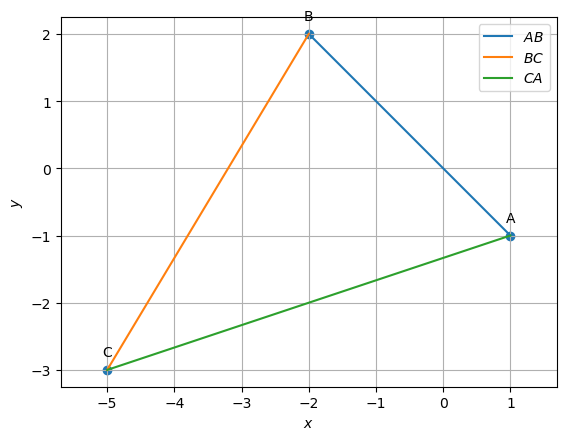
\includegraphics[width=\columnwidth]{./figs/Triangle.png}
\caption{triangle plotted using python}
\label{fig:i_triangle_py}
\end{figure}
\end{document}